\documentclass[tikz,border=10pt]{standalone}

\usepackage{tikz}
\usetikzlibrary{positioning}
\usetikzlibrary{shapes,arrows,backgrounds,fit,shapes.geometric,calc}
\usetikzlibrary{pgfplots.groupplots}
\usetikzlibrary{patterns}
\usepackage{pgfplots}
\usepackage{pgfplotstable}
\usepackage{listings}
\usepackage{lstautogobble}
\usepackage{color}

\renewcommand{\familydefault}{\sfdefault}

\lstset{
    language=[ANSI]C++,
    basicstyle=\small\ttfamily,
    identifierstyle=\color{black}\small\ttfamily,
    keywordstyle=\color{red}\small\ttfamily,
    commentstyle=\color{green!30!black}\bf\small\ttfamily,
    breaklines=true
}

\tikzset{
    %Define standard arrow tip
    >=stealth',
    % Define arrow style
    pil/.style={
           ->,
           color=black!60,
           thick,
           shorten <=2pt,
           shorten >=2pt,}
}
\newcommand{\mechnodewidth}{0.8cm}
\newcommand{\nodeheight}{1.5cm}
\newcommand{\lst}[1]{\lstinline!#1!}

\begin{document}
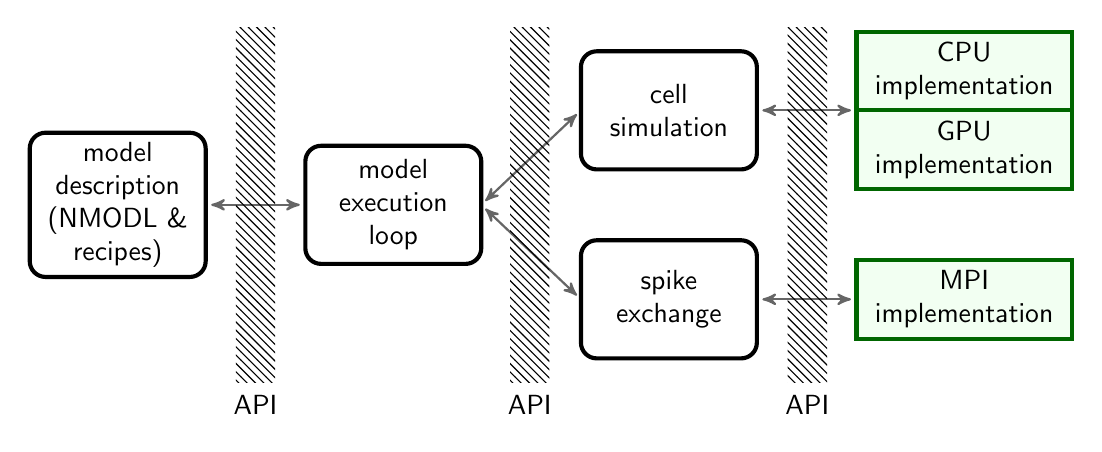
\begin{tikzpicture}[x=0cm, y=0cm, node distance=0 cm,outer sep = 0pt]
\tikzstyle{basicbox}=[draw=black, fill=white, rectangle, line width=1.5pt, rounded corners=2mm,
                   minimum height=\nodeheight, minimum width=2cm, text width=2cm, anchor=west, align=center]
\tikzstyle{widebox}=[draw=green!40!black, fill=green!5, rectangle, line width=1.5pt,
                   minimum height=1cm, minimum width=2.5cm, text width=2.5cm, anchor=west, align=center]
\tikzstyle{apibox}=[ fill=green, pattern=north west lines, rectangle,
                   minimum height=4.5cm, minimum width=0.5cm, align=center]

%%%%%%%%%%%%%%%%%%%%%%%%%%%%%%%%%
% NrnThread
%%%%%%%%%%%%%%%%%%%%%%%%%%%%%%%%%
    \node[basicbox] (desc) at (0.0cm,0.0cm) {model description\\ (NMODL \& \\ recipes)};
    \node[basicbox] (time) at (3.5cm,0.0cm) {model execution loop};
    \node[basicbox] (state)at (7.0cm,1.2cm) {cell\\simulation};
    \node[basicbox] (spike)at (7.0cm,-1.2cm) {spike\\exchange};
    \node[widebox] (cpu)  at (10.5cm,1.7cm) {CPU\\implementation};
    \node[widebox] (gpu)  at (10.5cm,0.7cm) {GPU\\implementation};
    \node[widebox] (cpu)  at (10.5cm,-1.2cm) {MPI\\implementation};

%\node[pointer] (time)    [right = 1.5cm of desc] {model exec loop};
%\node[pointer] (state)   [above right = 1cm of time] {cell simulation};
%\node[pointer] (spike)   [below right = 1cm of time] {spike exchange};
%\node[pointer] (cpu)     [above right = 1cm of state] {cpu implementation};
%\node[pointer] (gpu)     [below right = 1cm of state] {gpu implementation};

\path[pil,<->] (desc.east) edge (time.west);
\path[pil,<->] (time.east) edge (state.west);
\path[pil,<->] (time.east) edge (spike.west);
\path[pil,<->] (state.east) edge (10.5cm,1.2cm);
\path[pil,<->] (spike.east) edge (10.5cm,-1.2cm);

%\node[apibox] (api1)  at (2.5cm,0cm) {};
\node[apibox] (api1) at ($(desc)!0.5!(time)$) {};
\node[apibox] (api2) at (6.35cm,0cm) {};
\node[apibox] (api3) at (9.875cm,0cm) {};

\node[align=center] (apilabel) [below = 0.05cm of api1] {API};
\node[align=center] [below = 0.05cm of api2] {API};
\node[align=center] [below = 0.05cm of api3] {API};

%\tikzset{typeline/.style={draw=black!40, line width=2pt,
%                          inner sep=2mm, rectangle}};
%    \node (outline)[typeline, fit = (desc) (time) (spike) (state) (cpu)  (gpu) (apilabel) (api1)] {};

%\node at (outline.north west)
    %[anchor=south west, fill=white, draw=black!40, line width=2pt, minimum height=0.8cm, minimum width=4.5cm]
    %{\large {\texttt{Current Internal API}}};

\end{tikzpicture}
\end{document}

